\chapter{Le variabili}
{ }\hfill\textbf{Livello:} Principiante \\

Affrontiamo le variabili con esempio pratico. Qualche volta è necessario disegnare una figura in scala diversa. Per esempio se vogliamo disegnare un quadrato di lato pari a 100 passi, uno di lato pari a 200 ed un altro di lato pari a 50 dobbiamo scrivere tre diverse procedure, una per ciascun quadrato.

\begin{lstlisting}[caption="Il programma senza l'uso delle variabili"]
Per quadrato1
	Ripeti 4 [Avanti 100 RuotaDestra 90]
Fine
Per quadrato2
	Ripeti 4 [Avanti 200 RuotaDestra 90]
Fine
Per quadrato3
	Ripeti 4 [Avanti 50 RuotaDestra 90]
Fine
\end{lstlisting}

Capiamo immediatamente che sarebbe più semplice definire una sola procedura che riesca a disegnare tutti i tre quadrati e quadrati di qualsiasi lato. Per fare questo dobbiamo riuscire a dire alla procedura la lunghezza del lato del quadrato che vogliamo disegnare. Riusciamo a farlo grazie alle variabili, per esempio \texttt{quadrato 200} disegna un quadrato di lato 200 passi, \texttt{quadrato 100} disegna un quadrato di lato 100 e così via. Ma per fare ciò dobbiamo scrivere una procedura che sappia che vogliamo dirle quanto deve essere lungo il lato.



\section{Esempi}
\noindent La nostra procedura per disegnare il quadrato di lato 100 era:
\begin{lstlisting}
Per quadrato1
	Ripeti 4 [Avanti 100 RuotaDestra 90]
Fine
\end{lstlisting}  

Dobbiamo semplicemente modificare questa procedura in due punti:
\begin{enumerate}
	\item Aggiungiamo \texttt{:lato} alla fine della linea di definizione della procedura (riga 1). Questo dice all'interprete LOGO che la procedura si aspetta che le si dica la lunghezza del lato. \texttt{:lato} è chiamato l'argomento della procedura e definisce una variabile dello stesso nome che verrà riempita del valore della lunghezza del lato al momento di invocare la procedura stessa. 
	\item Sostituiamo la lunghezza del lato 100 con il nome della variabile \texttt{:lato}.
\end{enumerate}

Otteniamo:
\begin{lstlisting}[caption="Un programma per disegnare quadrati di qualsiasi lato"]
Per quadrato1 :lato
	Ripeti 4 [Avanti :lato RuotaDestra 90]
Fine
\end{lstlisting}

Quindi scrivendo \texttt{quadrato1 100 quadrato1 50 quadrato1 30 quadrato1 20 quadrato1 10} disegneremo la seguente figura:\\
\begin{center}
	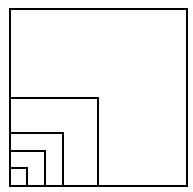
\includegraphics[scale=0.5]{pics/variables-carres.png}
\end{center}
\vspace{1cm}



\section{Disegnare un rettangolo delle dimensioni volute}
Definiamo una procedura chiamata \texttt{rec} che si aspetta due argomenti che rappresentano del dimensioni dei lati del rettangolo. Quindi \texttt{rec 200 100} dovrà disegnare un rettangolo di altezza 200 e lunghezza 100.
\begin{lstlisting}[caption="Rettangoli di qualiasi dimensione"]
Per rec :altezza :lunghezza
	Ripeti 2 [Avanti :altezza DX 90 Avanti :lunghezza DX 90]
end
\end{lstlisting} 

Alcuni disegni: 
\begin{lstlisting}
	rec 200 100 rec 100 300 rec 50 150 rec 1 20 rec 100 2 
\end{lstlisting}

Se invochiamo la procedura \texttt{rec} con solo un numero invece di due l'interprete LOGO fermerà il disegno e scriverà un messaggio di errore indicando che la procedura aspetta un secondo argomento.



\section{Disegnare in scale differenti}
Abbiamo imparato come disegnare un quadrato ed un rettangolo con lati diversi. Ora torniamo all'esempio della casa di pagina \pageref{maison} per modificare il programma per disegnare case di qualsiasi dimensione. \\
L'obiettivo è di invocare la procedura \texttt{casa} con un argomento che possa disegnare case più piccole o più grandi (la scala).
\begin{itemize}
	\item \texttt{casa 1} disegnerà la casa nelle dimensioni reali dei quadretti.
	\item \texttt{casa 0.5} disegnerà una casa grande la metà di quella originale.
	\item \texttt{casa 2} disegnerà una casa grande il doppio di quella originale.
\end{itemize}

Vediamo come modificare le singole procedure per accettare il fattore di scala. Originariamente la procedura quadrato era:
\begin{lstlisting}
Per quadrato
	Ripeti 4 [Avanti 150 RuotaDestra 90]
end
\end{lstlisting}

Tutte le dimensioni devono essere moltiplicate per la scala. Quindi la procedura del quadrato diventa:
\begin{lstlisting}[caption="Disegnare un quadrato in scala"]
	Ripeti 4 [Avanti 150*:scala RuotaDestra 90]
end
\end{lstlisting}

Quindi se invochiamo \texttt{quadrato 2}, il quadrato avrà i lati di lunghezza $150\times2=300$. Le proporzioni sono rispettate. Infatti vediamo che dobbiamo solo modificare le procedure sostituendo le lunghezze secondo questa regola:\\
\texttt{Av 70} diventa \texttt{Av 70*:scala} \\
\texttt{Av 45} diventa \texttt{Av 45*:scala} \\ 

\begin{lstlisting}[caption="Il disegno della casa in scala"]
per Quadrato :scala
	Ripeti 4[Avanti 150*:scala  RuotaDestra 90]
fine

per Triangolo :scala
	Ripeti 3[Avanti 150*:scala RuotaDestra 120]
fine

per Porta :scala
	Ripeti 2[Avanti 70*:scala RuotaDestra 90 
	Avanti 50*:scala RuotaDestra 90]
fine

per Camino :scala
	Avanti 55*:scala RuotaDestra 90 Avanti 20*:scala 
	RuotaDestra 90 Avanti 20*:scala
fine

per SpostaAB :scala
	RuotaDestra 90 Avanti 50*:scala RuotaSinistra 90
fine

per SpostaBC :scala
	RuotaSinistra 90 Avanti 50*:scala RuotaDestra 90 
	Avanti 150*:scala RuotaDestra 30
fine

per SpostaCD :scala
	PennaSu RuotaDestra 60 Avanti 20*:scala RuotaSinistra 90 
	Avanti 35*:scala PennaGiu
fine
\end{lstlisting}


\section{Esercizio}
Prova a generare i seguenti disegni a diverse scale.\\
\begin{center}
	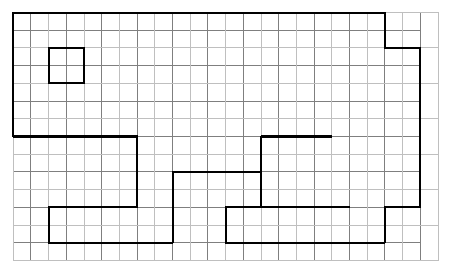
\includegraphics[scale=0.6]{pics/variables-grenouille.png}
\end{center}
\begin{center}
	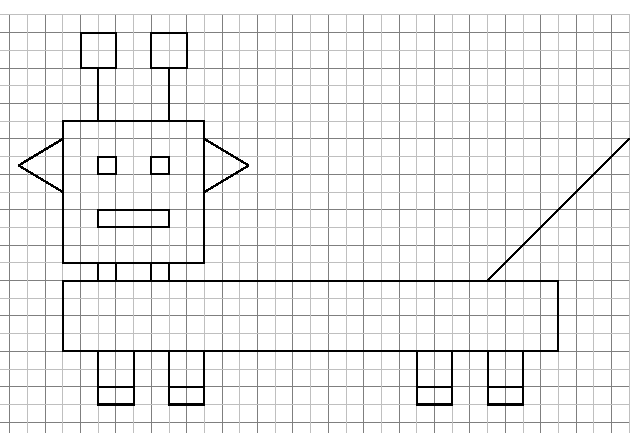
\includegraphics[scale=0.75]{pics/variables-robot.png}
\end{center}
